\chapterimage{back2.jpg} % Chapter heading image
\chapter{Combinatorial}

This first project introduces the combinatorial or asynchronous behaviour of the board. The outputs are updated as soon as the inputs are modified and not after a given period of time (a delay) which is a synchronous behaviour.\\
The equations that we would like to implement are:
\begin{center}
O$_0$ = I$_1$ and I$_2$ and I$_3$\\
O$_2$ = not(O$_1$)    
\end{center}
O$_1$ will be ON only when all inputs are ON, unless it will be OFF (the AND function over three Boolean values). 0$_2$ is the opposite of O$_1$: 0$_2$ is ON when O$_1$ is OFF, and OFF when O$_1$ is ON \footnote{This is a usual practice in the railways to detect if an equipment is failing or has not power supply. If both outputs are OFF, we know that the system is failing and the situation has to be handled with care.}.

\section{Modelling}

The modelling requires three steps:
\begin{itemize}
    \item The first step is to create a project, to give it a name and select "CSSP project".
    \item The second step is to add a board (only one) and to change the names of the inputs and outputs to respectively I1, I2, I3 and O1, O2.
    \item the third step is to modify the components \textit{logic} and \textit{logic\_i} to specify and implement the behaviour. 
\end{itemize}
 
 \lstset{frameround=fttt,keywordstyle=\color{ocre}\bfseries}
\lstinputlisting[language=B, frame=trbl, firstline=19,lastline=23,caption={Non-deterministic specification of the operation user\_logic},label=examples:combinatorial-spec, rulecolor=\color{ocre}]{chapterProjects/combinatorial_1_logic.mch}

For \textit{logic}, we need to modify the specification of the operation user\_logic. We could be precise and express directly the relationship between inputs and outputs, but for the very first experiment, we prefer to simply assert that the two outputs O1 and O2 are going to be modified non-deterministically\footnote{The var :: type substitution is called non-deterministic because a particular value is provided. In the implementation, the value assigned to the variable var should belong to uint8\_t. We remind you that the input and output digital values are represented by 8-bit values: IO\_OFF and IO\_ON.} (see listing \ref{examples:combinatorial-spec}). 

 \lstset{frameround=fttt,keywordstyle=\color{ocre}\bfseries}
\lstinputlisting[language=B, frame=trbl, firstline=24,lastline=49,caption={The implementation of the operation user\_logic},label=examples:combinatorial-impl, rulecolor=\color{ocre}]{chapterProjects/combinatorial_1_logic_i.imp}

For \textit{logic\_i}, the variables 01 and 02 are already defined as CONCRETE\\VARIABLES and both initialised with the value IO\_OFF. No other variable is required for the implementation. We only need to modify the body of the operation user\_logic (see listing \ref{examples:combinatorial-impl}). \\
We need three local variables to store the values of the three inputs I1, I2 and I3. So we define three variables i1\_, i2\_ and i3\_ with the substitution VAR ... IN ... END. The scope of this substitution in the END keyword, meaning that any use of these three variables outside of this scope will produce an error message. These three variables are typed prior to any use, by using the "becomes such that" substitution with the type uint8\_t. These three typing substitutions have no effect on the modelling but are required by the compiler.\\
The values of the inputs is collected by calling the three operations get\_I1, get\_I2 and get\_I3. The notation "var <-- op" means that the operation op is called and return one value that is assigned to the variable var. In our case, i1\_, i2\_ and i3\_ are valued respectively with the values returned by get\_I1, get\_I2 and get\_I3.
The next 8 lines represent the computation of O1: O1 is first set to IO\_OFF and then set to IO\_ON only if the three inputs are all equal to IO\_ON. 
\begin{remark}
The compiler in it current version does not support multiple testing conditions. Hence IF THEN ELSE have to be nested. 
\end{remark}
Finally O2 is computed with the last IF THEN ELSE, based on the value computed for O1.
\begin{remark}
The sequence operator ; is not a line terminator like in C. Its role inside an operation\footnote{It is also used to separate operations} is to separate two substitutions. If extra ; are inserted in the model, error messages will be emitted when checking the model. 
\end{remark}

\section{Executing}

Now that the modelling is complete, we first need to check and prove the model. Select all the components by clicking on the central pane of the main window\footnote{the one showing all the components of the project.}, then type ctrl+A. Type ctrl+0 to initiate the typecheck, proof obligation generation and proof of all these components. If some mistake was made, error messages are displayed either in the model editor or the error/warning pane in the main window. Be sure to correct any mistake before moving on. Finally press ctrl+U to complete the proof. You should obtain the proof status of the figure \ref{projects:Combinatorial_1-project-status} (the Unproved column shows only zeros, meaning that the project is fully proved).
\begin{figure}[h]
\centering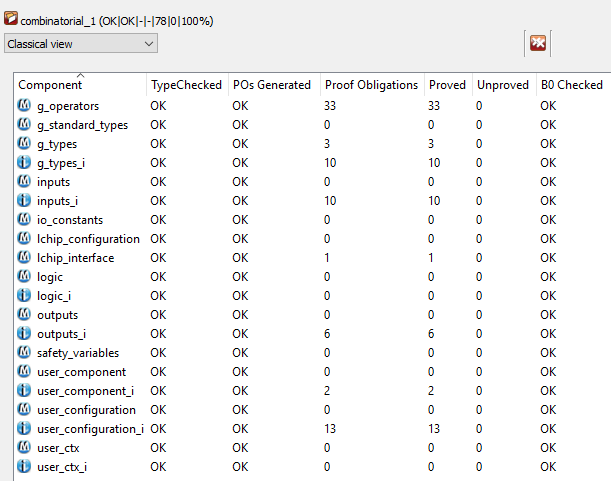
\includegraphics[scale=0.5]{Pictures/chaptProjects/comb1-project-status.png}
\caption{Combinatorial\_1 project status}
\label{projects:Combinatorial_1-project-status}
\end{figure}
The project is ready to be compiled. Be sure that your SK0 board is connected with the USB connector to your host. Right-click on the project name in the left pane and select "CSSP Runner". A new window appears, showing a carousel of all the steps of the compilation. Click on the green triangle on the top left. All steps are cleared until the last one where you are asked to reset the SK0 board. Use a pen to push on the reset button and release it. The board starts to blink as it enters bootload mode. After around 30s, the last step is cleared (green check) and you are again invited to reset the SK0 board. Push the reset button and release it. After 2 seconds, the board starts to execute your program.

\section{Testing}

To test your program, you need to be able to modify the status of the inputs in order to change the status of the outputs. You need three switches or three wires that you could plug/unplug to open/close the input circuits. The switches have to be connected to the two right pins as shown on figure \ref{projects:Combinatorial_1-connecting}.
\begin{figure}[h]
\centering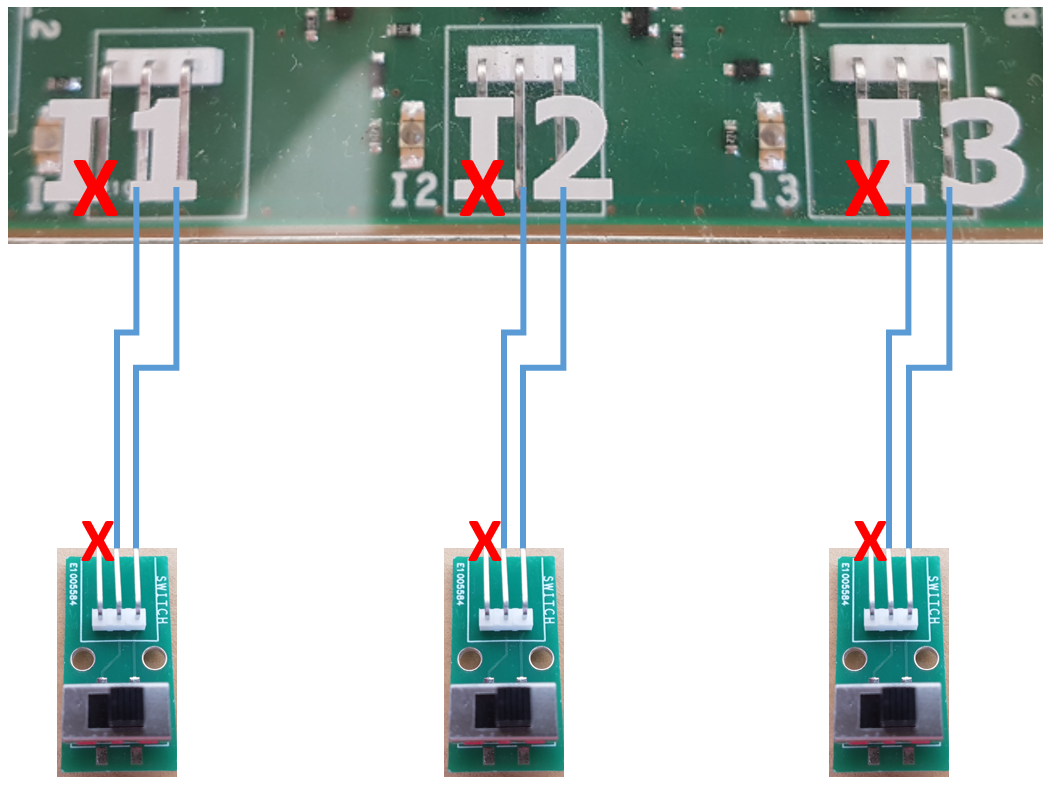
\includegraphics[scale=0.25]{Pictures/chaptProjects/combinatorial-montage.png}
\caption{Connecting switches to the board}
\label{projects:Combinatorial_1-connecting}
\end{figure}
The status of the three inputs is indicated by three LEDs. One LED is ON when enough current is provided through the input circuit, OFF if not. \\
Connect your switches, change their status and see how the behaviour evolves. You should get the configurations shown in figure \ref{projects:Combinatorial_1-connecting}.
\begin{figure}[h]
\centering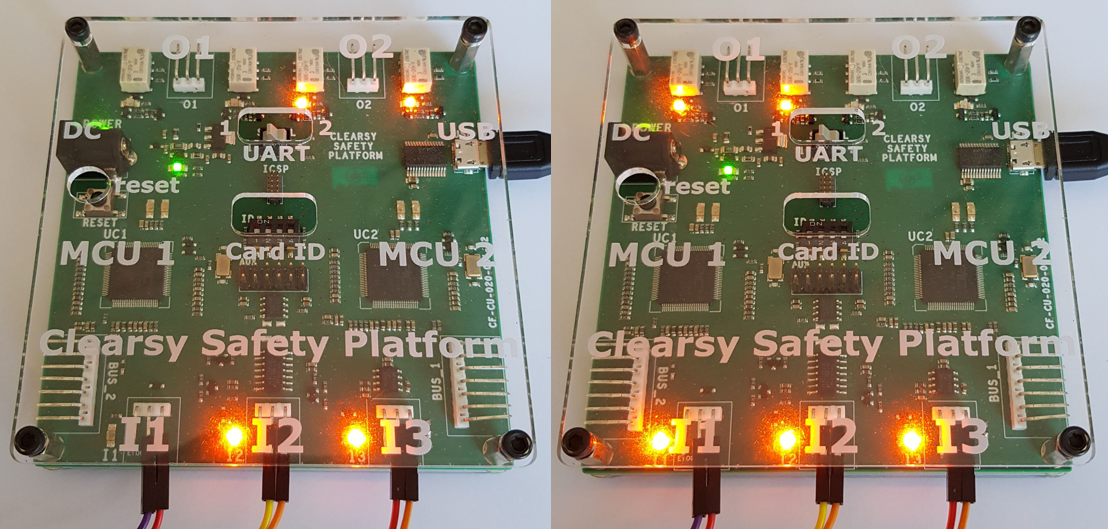
\includegraphics[scale=0.5]{Pictures/chaptProjects/comb1_join.png}
\caption{Two configurations: not all inputs are ON (left) and only O2 is ON; all inputs are ON (right) and only O1 is ON.}
\label{projects:Combinatorial_1-connecting}
\end{figure}

\begin{exercise}
Create a program which implements the following equations:
\begin{center}
O$_0$ = I$_1$ or I$_2$ or I$_3$\\
O$_2$ = not(O$_1$)    
\end{center}
First create a new project and populate it with models similar to combinatorial\_1. Then modify the body of the operation user\_logic in the component \textit{logic\_i} to implement a disjunction over the values of the three inputs.
\end{exercise}